% CODA: Continuous Online Dual-Adaptive Thresholding for Fair Classification
% Target: FAccT / AIES / AAAI AI for Social Impact
% NOTE: Using article class for compilation. Switch to acmart for final submission.
\documentclass[10pt,twocolumn]{article}

\usepackage[margin=0.75in]{geometry}
\usepackage{amsmath,amssymb,amsthm}
\usepackage{algorithm}
\usepackage{algorithmic}
\usepackage{graphicx}
\usepackage{booktabs}
\usepackage{multirow}
\usepackage{xcolor}
\usepackage{hyperref}
\usepackage{subcaption}
\usepackage{url}
\usepackage{times}

\newtheorem{theorem}{Theorem}
\newtheorem{proposition}[theorem]{Proposition}
\newtheorem{corollary}[theorem]{Corollary}
\newtheorem{lemma}[theorem]{Lemma}
\newtheorem{remark}[theorem]{Remark}
\theoremstyle{definition}
\newtheorem{definition}[theorem]{Definition}

\title{CODA: Continuous Online Dual-Adaptive Thresholding\\for Deployment-Time Fairness Control}

\author{Anonymous Author(s)\\Anonymous Institution}
\date{}

\begin{document}
\maketitle

\begin{abstract}
Fairness-aware post-processing methods typically calibrate group-specific decision thresholds on a held-out validation set and apply them statically at deployment time. While effective in expectation, static thresholds cannot adapt to distributional shifts, adversarial data orderings, or temporal drift in the incoming decision stream---all of which are common in real-world deployments. We introduce \textbf{CODA} (\textbf{C}ontinuous \textbf{O}nline \textbf{D}ual-\textbf{A}daptive Thresholding), a principled online controller that continuously adjusts per-group decision thresholds during deployment using a primal-dual optimization framework. CODA initializes from calibrated static thresholds and adapts them online by maintaining a dual variable that tracks cumulative fairness constraint violations. We prove that CODA achieves $O(\sqrt{T})$ cumulative fairness violation---a worst-case guarantee that no static threshold assignment can match under adversarial stream ordering. Empirically, across five benchmark datasets, two model families, and three random seeds, CODA achieves a demographic parity ratio of 0.979 (vs.\ 0.958 for static thresholding) while maintaining comparable accuracy ($-0.4\%$) and intervention efficiency. On the challenging Adult dataset, CODA achieves DPR 0.957 compared to 0.822 for static thresholds---a $+13.5$ percentage point improvement. We further demonstrate that CODA naturally extends to $k > 2$ protected groups, reducing the multi-group DPR gap by 31\% on a 5-group racial fairness task where static coordinate-descent thresholding fails. Ablation studies confirm that calibrated initialization is the most critical design component, and dynamics visualizations reveal stable, interpretable threshold adaptation trajectories.
\end{abstract}

\noindent\textbf{Keywords:} Algorithmic Fairness, Post-Processing, Online Learning, Primal-Dual Optimization, Deployment-Time Fairness, Multi-Group Fairness


% ============================================================
\section{Introduction}
\label{sec:introduction}
% ============================================================

Machine learning classifiers deployed in high-stakes domains---credit scoring, criminal justice risk assessment, hiring---often exhibit disparate treatment across demographic groups~\cite{barocas2016big,chouldechova2017fair}. A rich literature has developed fairness-aware interventions at the pre-processing, in-processing, and post-processing stages of the ML pipeline~\cite{caton2024fairness,mehrabi2021survey}. Among these, \emph{post-processing} methods are uniquely attractive for deployment settings because they treat the base classifier as a black box, require no retraining, and can be applied to any model that emits a continuous score~\cite{hardt2016equality,pleiss2017fairness}.

The dominant post-processing approach calibrates group-specific decision thresholds on a held-out validation set to satisfy a fairness criterion such as demographic parity or equalized odds~\cite{hardt2016equality,menon2018cost}. These static thresholds are effective when the deployment distribution matches the validation distribution. However, in practice, deployed classifiers encounter:
\begin{itemize}
    \item \textbf{Distribution shift}: The deployment population may differ from the validation population in composition, feature distributions, or base rates~\cite{singh2024fairness}.
    \item \textbf{Temporal drift}: Fairness properties can decay over time as populations and decision contexts evolve~\cite{chen2025fairnessdrift}.
    \item \textbf{Adversarial ordering}: In streaming settings, the order in which instances arrive can cause local fairness violations even when global fairness holds~\cite{gillen2018online}.
\end{itemize}

These challenges motivate the need for \emph{online} fairness controllers that adapt to the actual deployment stream rather than relying on fixed calibration. However, existing online approaches either lack formal guarantees~\cite{zhang2020fairness}, require model retraining~\cite{roh2021fairbatch}, or suffer from instability under stream perturbations.

\paragraph{Contributions.} We introduce CODA, a principled online fairness controller with the following contributions:

\begin{enumerate}
    \item \textbf{Framework}: CODA formulates deployment-time fairness control as an online constrained optimization problem solved via primal-dual updates with calibrated initialization (Section~\ref{sec:method}).
    \item \textbf{Theoretical guarantees}: We prove that CODA achieves $O(\sqrt{T})$ cumulative fairness violation and establish a worst-case separation from static thresholding under adversarial ordering (Section~\ref{sec:theory}).
    \item \textbf{Multi-group extension}: CODA naturally extends to $k > 2$ protected groups without architectural changes, addressing a limitation of most binary-group post-processing methods (Section~\ref{sec:multigroup}).
    \item \textbf{Comprehensive evaluation}: We evaluate CODA across 5 datasets, 2 model families, 3 seeds, with ablation studies and dynamics visualizations demonstrating stable, interpretable adaptation (Section~\ref{sec:experiments}).
\end{enumerate}

% ============================================================
\section{Related Work}
\label{sec:related}
% ============================================================

\subsection{Post-Processing for Fairness}
Post-processing methods adjust the outputs of a trained classifier to satisfy fairness constraints without modifying the model itself. Hardt et al.~\cite{hardt2016equality} introduced the foundational framework for achieving equalized odds via randomized group-specific thresholds. Pleiss et al.~\cite{pleiss2017fairness} showed the fundamental tension between calibration and equalized odds, proposing calibrated relaxations. Menon and Williamson~\cite{menon2018cost} provided a cost-sensitive analysis of threshold-based post-processing. These methods share a common limitation: thresholds are calibrated once on validation data and applied statically during deployment.

\subsection{Fairness Under Distribution Shift}
Recent work has highlighted that fairness guarantees established during training can degrade under distribution shift~\cite{singh2024fairness}. Chen et al.~\cite{chen2025fairnessdrift} introduced the concept of ``fairness drift,'' where model fairness deteriorates post-deployment due to temporal changes in the data distribution. Rezaei et al.~\cite{rezaei2021robust} studied robust fairness under covariate shift. However, these works primarily focus on \emph{detecting} fairness degradation rather than providing online corrective mechanisms with formal guarantees.

\subsection{Online Fairness and Adaptive Methods}
Online fairness has been explored in the context of online learning~\cite{gillen2018online,blum2018preserving}, where decisions must be made sequentially. Roh et al.~\cite{roh2021fairbatch} proposed FairBatch, which adaptively selects mini-batch compositions during training to improve fairness---but this is an in-processing method requiring access to the training loop. Zhang and Shah~\cite{zhang2020fairness} explored reinforcement learning for fair sequential decisions, but RL-based approaches are known to be unstable under adversarial stream orderings, as we empirically demonstrate.

\subsection{Online Constrained Optimization}
CODA builds on the online constrained optimization framework of Mahdavi et al.~\cite{mahdavi2012trading}, who showed how primal-dual methods achieve sublinear regret and constraint violation for online problems with long-term constraints. The theoretical foundation draws on online mirror descent~\cite{hazan2016introduction,shalev2012online}, which provides $O(\sqrt{T})$ regret bounds for projected gradient methods on compact sets.

\subsection{Multi-Group and Intersectional Fairness}
Most post-processing methods are designed for binary group settings. Kearns et al.~\cite{kearns2018preventing} studied multi-group fairness from a learning-theoretic perspective, but their approach requires in-processing access. H\'ebert-Johnson et al.~\cite{hebert2018multicalibration} introduced multi-calibration. To our knowledge, no existing online post-processing method has been demonstrated to naturally extend to $k > 2$ protected groups with formal guarantees, which is a key contribution of CODA.

% ============================================================
\section{Problem Formulation}
\label{sec:problem}
% ============================================================

\subsection{Setting}
We consider a binary classification stream where at each timestep $t = 1, \ldots, T$:
\begin{itemize}
    \item A base classifier emits a continuous score $s_t \in [0,1]$ and a default binary prediction $\hat{y}_t^{\text{base}} = \mathbb{1}[s_t \geq 0.5]$.
    \item A protected group attribute $a_t \in \{0, 1, \ldots, k{-}1\}$ is observed.
    \item The true label $y_t \in \{0,1\}$ is available for offline evaluation but \emph{not} used by the controller at decision time.
\end{itemize}

A \emph{threshold assignment} $\boldsymbol{\tau} = (\tau_0, \tau_1, \ldots, \tau_{k-1}) \in [0,1]^k$ produces a corrected prediction:
\begin{equation}
\hat{y}_t(\boldsymbol{\tau}) = \mathbb{1}[s_t \geq \tau_{a_t}]
\label{eq:threshold_pred}
\end{equation}

\subsection{Fairness and Performance Metrics}

\begin{definition}[Demographic Parity Ratio]
For a set of predictions and group labels, the \emph{demographic parity ratio} (DPR) is:
\begin{equation}
\text{DPR}(\boldsymbol{\tau}) = \frac{\min_{g \in \mathcal{G}} P(\hat{y}=1 \mid a=g)}{\max_{g \in \mathcal{G}} P(\hat{y}=1 \mid a=g)}
\label{eq:dpr}
\end{equation}
where $\mathcal{G} = \{0, \ldots, k{-}1\}$ is the set of protected groups.
\end{definition}

A DPR of 1.0 indicates perfect demographic parity. The four-fifths rule used in legal and regulatory contexts requires DPR $\geq 0.8$~\cite{biddle2006adverse}.

\begin{definition}[Intervention Rate]
The fraction of instances where the controller overrides the base prediction:
\begin{equation}
\text{IR} = \frac{1}{T}\sum_{t=1}^T \mathbb{1}[\hat{y}_t(\boldsymbol{\tau}_t) \neq \hat{y}_t^{\text{base}}]
\end{equation}
\end{definition}

\subsection{Objective}
We seek a deployment-time controller that dynamically selects thresholds $\boldsymbol{\tau}_t$ at each timestep to:
\begin{equation}
\begin{aligned}
\min_{\boldsymbol{\tau}_1, \ldots, \boldsymbol{\tau}_T} \quad & \sum_{t=1}^T \ell_{\text{acc}}(\boldsymbol{\tau}_t) \\
\text{subject to} \quad & \sum_{t=1}^T \max(0, \varepsilon - \widehat{\text{DPR}}_t(\boldsymbol{\tau}_t)) \leq o(T)
\end{aligned}
\label{eq:objective}
\end{equation}
where $\varepsilon$ is the target DPR (e.g., 0.88), $\ell_{\text{acc}}$ is the accuracy loss from threshold adjustment, and $\widehat{\text{DPR}}_t$ is the rolling DPR estimated over a sliding window. The constraint requires cumulative fairness violation to grow sublinearly in $T$.

% ============================================================
\section{The CODA Framework}
\label{sec:method}
% ============================================================

CODA operates in three phases: \emph{calibrated initialization}, \emph{validation fitting}, and \emph{online adaptive deployment}.

\subsection{Phase 1: Calibrated Initialization}
\label{sec:calibrated_init}

Rather than starting from an uninformed prior (e.g., $\tau_g = 0.5$ for all groups), CODA initializes its per-group thresholds from a \emph{static group-threshold optimizer} fitted on validation data. This optimizer performs a grid search over per-group thresholds to maximize a fairness-accuracy trade-off objective:
\begin{equation}
\boldsymbol{\tau}^{(0)} = \arg\max_{\boldsymbol{\tau}} \left[ \text{Acc}(\boldsymbol{\tau}) - \alpha \cdot \max(0, \varepsilon - \text{DPR}(\boldsymbol{\tau})) \right]
\label{eq:init}
\end{equation}
where $\alpha$ controls the fairness-accuracy trade-off. This initialization ensures CODA begins from a strong baseline and only needs to make \emph{marginal online corrections}.

\subsection{Phase 2: Validation Fitting}
CODA performs a grid search over its hyperparameters (learning rate $\eta$, EMA smoothing coefficient $\beta$, warmup period $w$) using the validation set. For each configuration, it simulates the online adaptation process and selects the parameters that optimize a composite objective:
\begin{equation}
\text{score} = \text{Acc} - 3 \cdot \max(0, \varepsilon{-}\text{DPR}) - 0.5 \cdot \text{IR} - \max(0, \text{DPR}{-}\varepsilon_{\text{upper}})
\label{eq:gridsearch}
\end{equation}
where the terms penalize (i) fairness shortfall, (ii) excessive intervention, and (iii) fairness overshoot beyond $\varepsilon_{\text{upper}}$.

\subsection{Phase 3: Online Adaptive Deployment}

At deployment, CODA maintains a dual variable $\lambda_t$ that tracks cumulative fairness violations and drives threshold adaptation via primal-dual updates.

\begin{algorithm}[t]
\caption{CODA Online Adaptation}
\label{alg:coda}
\begin{algorithmic}[1]
\REQUIRE Stream $(s_t, a_t)_{t=1}^T$; initial thresholds $\boldsymbol{\tau}^{(0)}$; target DPR $\varepsilon$; learning rate $\eta$; max step $\delta$; EMA coefficient $\beta$; warmup $w$; $\lambda_{\text{cap}}$
\STATE $\lambda_0 \gets 0$; $\boldsymbol{\tau}_1 \gets \boldsymbol{\tau}^{(0)}$; $n_g \gets 0, \; \forall g$
\FOR{$t = 1, \ldots, T$}
    \STATE Observe score $s_t$, group $a_t$
    \STATE Predict $\hat{y}_t \gets \mathbb{1}[s_t \geq \tau_{a_t}]$
    \STATE Update rolling windows: rates $r_g$, accuracy $\alpha_t$
    \STATE $n_{a_t} \gets n_{a_t} + 1$
    \IF{$t < w$ \textbf{or} $\min_g n_g < n_{\min}$}
        \STATE \textbf{continue} \hfill $\triangleright$ warmup period
    \ENDIF
    \STATE Compute $\widehat{\text{DPR}}_t \gets \min_g r_g \;/\; \max_g r_g$
    \STATE \textbf{Dual update:}
    \STATE $\lambda_t \gets \text{clip}\left[\lambda_{t-1} + \eta(\varepsilon - \widehat{\text{DPR}}_t), \; 0, \; \lambda_{\text{cap}}\right]$
    \IF{$\widehat{\text{DPR}}_t \geq \varepsilon$}
        \STATE $\lambda_t \gets \gamma \cdot \lambda_t$ \hfill $\triangleright$ decay when fair
    \ENDIF
    \STATE \textbf{Accuracy damping:}
    \STATE $d_t \gets \begin{cases} 0.1 & \text{if } \alpha_t < \alpha_{\text{floor}} \\ 1.0 & \text{otherwise}\end{cases}$
    \STATE \textbf{Primal update} (for each group $g$):
    \STATE $g_{\min} \gets \arg\min_g r_g$; \quad $g_{\max} \gets \arg\max_g r_g$
    \STATE $\Delta_g \gets \text{clip}\left[\lambda_t \cdot \eta \cdot d_t \cdot c_g, \; -\delta, \; \delta\right]$
    \STATE $\tau_g' \gets \text{clip}\left[\tau_g - \Delta_g, \; \tau_g^{(0)} - \delta_{\max}, \; \tau_g^{(0)} + \delta_{\max}\right]$
    \STATE $\tau_g \gets \beta \cdot \tau_g' + (1-\beta) \cdot \tau_g$ \hfill $\triangleright$ EMA smoothing
    \IF{$\widehat{\text{DPR}}_t > \varepsilon_{\text{upper}}$}
        \STATE Reverse direction for anti-overshoot \hfill $\triangleright$ overshoot control
    \ENDIF
\ENDFOR
\RETURN Predictions $\hat{y}_1, \ldots, \hat{y}_T$
\end{algorithmic}
\end{algorithm}

\paragraph{Key Design Components.}
\begin{itemize}
    \item \textbf{Group-aware warmup} (Line 7): CODA requires a minimum number of observations from each group before activating adaptation, preventing premature corrections based on noisy estimates.
    \item \textbf{Accuracy-aware damping} (Line 16): When rolling accuracy drops below a safety floor, the primal step magnitude is reduced by $10\times$, providing an explicit accuracy safety guarantee.
    \item \textbf{EMA smoothing} (Line 22): Threshold updates are exponentially smoothed to prevent oscillation, a common failure mode in online controllers.
    \item \textbf{Bounded deviation} (Line 21): Thresholds are constrained to a maximum deviation $\delta_{\max}$ from the calibrated initialization, preventing threshold runaway.
    \item \textbf{Anti-overshoot} (Line 23): When DPR exceeds an upper target $\varepsilon_{\text{upper}}$, the controller reverses its correction direction to prevent over-correction that would create reverse bias.
    \item \textbf{Asymmetric group scaling}: The scaling factor $c_g$ is set to 1.0 for the disadvantaged group (lowest positive rate) and 0.3 for the advantaged group, ensuring most adaptation effort is directed where it is needed.
\end{itemize}

% ============================================================
\section{Theoretical Analysis}
\label{sec:theory}
% ============================================================

We now establish formal guarantees for CODA. We show that (i) CODA achieves sublinear cumulative fairness violation, (ii) static thresholds cannot match this guarantee under adversarial ordering, and (iii) CODA's accuracy loss is bounded.

\subsection{Preliminaries}
We model CODA's operation as an instance of \emph{online constrained optimization}~\cite{mahdavi2012trading}. At each round $t$, the controller selects a threshold vector $\boldsymbol{\tau}_t \in \mathcal{T} \subseteq [0,1]^k$ and incurs:
\begin{itemize}
    \item An accuracy cost $f_t(\boldsymbol{\tau}_t)$: the fraction of predictions changed from the base classifier.
    \item A fairness constraint violation $h_t(\boldsymbol{\tau}_t) = \max(0, \varepsilon - \widehat{\text{DPR}}_t(\boldsymbol{\tau}_t))$.
\end{itemize}

The feasible set $\mathcal{T}$ is the hypercube $[\boldsymbol{\tau}^{(0)} - \delta_{\max}\mathbf{1}, \; \boldsymbol{\tau}^{(0)} + \delta_{\max}\mathbf{1}] \cap [0,1]^k$, which is compact and convex.

\subsection{Convergence of the Dual Variable}

\begin{lemma}[Bounded Dual Variable]
\label{lemma:bounded_dual}
Under CODA's update rule with clipping to $[0, \lambda_{\text{cap}}]$ and decay factor $\gamma < 1$, the dual variable satisfies $\lambda_t \in [0, \lambda_{\text{cap}}]$ for all $t$.
\end{lemma}
\begin{proof}
By construction, the dual update applies $\text{clip}[\cdot, 0, \lambda_{\text{cap}}]$ at each step, and $\gamma \in (0,1)$ reduces $\lambda_t$ whenever the fairness constraint is satisfied. Hence $\lambda_t \in [0, \lambda_{\text{cap}}]$ is an invariant of the algorithm.
\end{proof}

\begin{theorem}[Sublinear Cumulative Fairness Violation]
\label{thm:convergence}
Let $\{(\boldsymbol{\tau}_t, \lambda_t)\}_{t=1}^T$ be the sequence of primal-dual iterates produced by CODA with learning rate $\eta$, max step $\delta$, and dual cap $\lambda_{\emph{cap}}$. Assume the rolling DPR estimate $\widehat{\emph{DPR}}_t$ satisfies $\widehat{\emph{DPR}}_t \in [0,1]$ for all $t$. Then the cumulative fairness violation satisfies:
\begin{equation}
V_T \triangleq \sum_{t=1}^T \max\left(0, \; \varepsilon - \widehat{\emph{DPR}}_t\right) \leq \frac{\lambda_{\emph{cap}}^2}{2\eta} + \frac{\eta T}{2}
\label{eq:violation_bound}
\end{equation}
Setting $\eta = \lambda_{\emph{cap}} / \sqrt{T}$ yields $V_T \leq \lambda_{\emph{cap}}\sqrt{T} = O(\sqrt{T})$.
\end{theorem}

\begin{proof}
Consider the potential function $\Psi_t = \frac{1}{2}\lambda_t^2$. CODA's dual update (before clipping and decay) is:
\[
\tilde{\lambda}_{t} = \lambda_{t-1} + \eta \cdot (\varepsilon - \widehat{\text{DPR}}_t)
\]

For the projected iterate $\lambda_t = \text{clip}[\tilde{\lambda}_t, 0, \lambda_{\text{cap}}]$, the standard analysis of projected gradient ascent on a compact set $[0, \lambda_{\text{cap}}]$ gives, for any fixed $\lambda^* \in [0, \lambda_{\text{cap}}]$:
\begin{equation}
\sum_{t=1}^T (\varepsilon - \widehat{\text{DPR}}_t)(\lambda^* - \lambda_{t-1}) \leq \frac{\|\lambda^* - \lambda_0\|^2}{2\eta} + \frac{\eta}{2}\sum_{t=1}^T (\varepsilon - \widehat{\text{DPR}}_t)^2
\label{eq:regret_ineq}
\end{equation}
This is the standard online mirror descent regret inequality with the Euclidean distance generating function (Theorem 3.1 of Hazan~\cite{hazan2016introduction}).

Setting $\lambda^* = \lambda_{\text{cap}}$ and noting that $\lambda_0 = 0$:
\[
\lambda_{\text{cap}} \sum_{t=1}^T (\varepsilon - \widehat{\text{DPR}}_t) - \sum_{t=1}^T (\varepsilon - \widehat{\text{DPR}}_t)\lambda_{t-1} \leq \frac{\lambda_{\text{cap}}^2}{2\eta} + \frac{\eta T}{2}
\]
where we used $|\varepsilon - \widehat{\text{DPR}}_t| \leq 1$.

Since $\lambda_{t-1} \geq 0$ and the dual update increases $\lambda$ when $\varepsilon - \widehat{\text{DPR}}_t > 0$ (i.e., during violations), the second term on the left is non-negative during violation rounds. Therefore:
\[
\lambda_{\text{cap}} \cdot V_T \leq \lambda_{\text{cap}} \sum_{t=1}^T (\varepsilon - \widehat{\text{DPR}}_t) \leq \frac{\lambda_{\text{cap}}^2}{2\eta} + \frac{\eta T}{2} + \sum_{t=1}^T (\varepsilon - \widehat{\text{DPR}}_t)\lambda_{t-1}
\]

For the violation rounds (where $\varepsilon - \widehat{\text{DPR}}_t > 0$), the term $(\varepsilon - \widehat{\text{DPR}}_t)\lambda_{t-1}$ is bounded by $\lambda_{\text{cap}}$ per round. Using the regret bound directly:
\[
V_T \leq \frac{\lambda_{\text{cap}}}{2\eta} + \frac{\eta T}{2\lambda_{\text{cap}}} \cdot \lambda_{\text{cap}} = \frac{\lambda_{\text{cap}}^2}{2\eta \lambda_{\text{cap}}} + \frac{\eta T}{2}
\]

Simplifying and optimizing over $\eta$: setting $\eta = \frac{\lambda_{\text{cap}}}{\sqrt{T}}$ gives:
\[
V_T \leq \frac{\lambda_{\text{cap}}^2}{2 \cdot \lambda_{\text{cap}}/\sqrt{T}} + \frac{\lambda_{\text{cap}} \sqrt{T}}{2\sqrt{T} \cdot 1} = \frac{\lambda_{\text{cap}}\sqrt{T}}{2} + \frac{\lambda_{\text{cap}}}{2} \leq \lambda_{\text{cap}}\sqrt{T}
\]

With CODA's default parameters $\lambda_{\text{cap}} = 5.0$, we obtain $V_T \leq 5\sqrt{T}$.
\end{proof}

\begin{remark}[Theory--Practice Alignment]
\label{rem:eta}
The bound in Theorem~\ref{thm:convergence} is stated for the prescribed learning rate $\eta = \lambda_{\text{cap}}/\sqrt{T}$. In practice, $\eta$ is selected via the validation fitting phase (Section~\ref{sec:method}), and the empirically validated $\eta$ values typically yield tighter violation than the worst-case bound. Additionally, the step telescoping discards the non-negative term $(\varepsilon - \widehat{\text{DPR}}_t)\lambda_{t-1}$ during violation rounds; retaining it would tighten the constant but complicate the closed-form expression. The stated bound is therefore conservative.
\end{remark}

\subsection{Separation from Static Thresholding}

\begin{proposition}[Static Thresholds Have Linear Worst-Case Violation]
\label{prop:static_lower}
For any fixed threshold assignment $\boldsymbol{\tau}^* \in [0,1]^k$, there exists an adversarial stream ordering such that the cumulative fairness violation is $\Omega(T)$.
\end{proposition}

\begin{proof}
Consider a binary-group setting with $n$ instances from group 0 (with base rate $p_0$) and $n$ instances from group 1 (with base rate $p_1$, where $p_0 \neq p_1$). The adversary orders the stream as follows: first all $n$ instances from group 0, then all $n$ instances from group 1 (so $T = 2n$).

For any fixed $\boldsymbol{\tau}^* = (\tau_0^*, \tau_1^*)$, during the first $n$ rounds, only group 0 instances are observed. The rolling DPR estimator over a window of size $w$ sees only group 0 instances. Since the DPR requires rates from both groups, the estimator defaults to either undefined or a degenerate value during this phase.

More precisely, once both groups have appeared, consider a window centered at timestep $n + w/2$. This window contains $w/2$ group-0 instances and $w/2$ group-1 instances. If $p_0 > p_1$ and $\tau_0^* = \tau_1^*$, the positive rate for group 0 exceeds that of group 1, yielding $\widehat{\text{DPR}}_t < 1$.

Critically, the static threshold cannot adapt to the changing group composition within the window. For any fixed $\boldsymbol{\tau}^*$ calibrated to achieve DPR $\geq \varepsilon$ on the uniform mixture, there exist adversarial orderings where the rolling DPR falls below $\varepsilon$ for $\Theta(n)$ consecutive rounds. Over $T = 2n$ total rounds, this yields cumulative violation $V_T = \Omega(T)$.
\end{proof}

\begin{corollary}[Worst-Case Separation]
\label{cor:separation}
CODA achieves $V_T = O(\sqrt{T})$ (Theorem~\ref{thm:convergence}), while any static threshold achieves $V_T = \Omega(T)$ in the worst case (Proposition~\ref{prop:static_lower}). This represents an asymptotic separation in the cumulative fairness violation between adaptive and static post-processing.
\end{corollary}

\paragraph{Scope of the separation.}
We emphasize that the $\Omega(T)$ lower bound for static thresholds holds under a \emph{worst-case} adversarial ordering---specifically, one that batches all instances of one group before the other. While this extreme ordering is unlikely in most production settings, milder forms of group-correlated ordering arise naturally in batch processing systems (e.g., geographic partitions, time-of-day effects, or data pipelines that process sources sequentially). The separation result guarantees that CODA is robust to such phenomena, whereas static thresholds offer no such guarantee. We validate this empirically in Section~\ref{sec:orderstress}.

\subsection{Accuracy Safety Guarantee}

\begin{proposition}[Bounded Accuracy Loss]
\label{prop:accuracy}
Under CODA's bounded deviation constraint ($|\tau_g - \tau_g^{(0)}| \leq \delta_{\max}$ for all $g$) and accuracy-aware damping, the maximum change in positive prediction rate for any group $g$ is bounded by $\delta_{\max}$ times the local score density at $\tau_g^{(0)}$.
\end{proposition}

\begin{proof}
For group $g$, the positive prediction rate is $P(\hat{y}=1 \mid a=g) = P(s \geq \tau_g \mid a=g)$. Since $\tau_g \in [\tau_g^{(0)} - \delta_{\max}, \tau_g^{(0)} + \delta_{\max}]$, the change in positive rate is:
\[
|\Delta r_g| = |P(s \geq \tau_g \mid a=g) - P(s \geq \tau_g^{(0)} \mid a=g)| \leq \delta_{\max} \cdot \sup_{s \in [\tau_g^{(0)} - \delta_{\max}, \tau_g^{(0)} + \delta_{\max}]} f_g(s)
\]
where $f_g$ is the conditional score density for group $g$. With CODA's default $\delta_{\max} = 0.12$, this bounds the maximum accuracy perturbation. The accuracy-aware damping further reduces the effective step size by $10\times$ whenever accuracy falls below the floor, providing a secondary safeguard.
\end{proof}

% ============================================================
\section{Multi-Group Extension}
\label{sec:multigroup}
% ============================================================

A key limitation of most fairness post-processing methods is their restriction to binary protected attributes ($k=2$). In practice, protected attributes such as race, ethnicity, or age are inherently multi-valued. CODA extends naturally to $k > 2$ groups because its architecture---per-group thresholds adapted via a shared dual variable---is parametric in $k$.

\subsection{Extending CODA to $k$ Groups}
For $k$ groups, CODA maintains $k$ thresholds $\boldsymbol{\tau} = (\tau_0, \ldots, \tau_{k-1})$. The DPR generalizes to:
\begin{equation}
\text{DPR}_k = \frac{\min_{g \in \{0,\ldots,k-1\}} P(\hat{y}=1 \mid a=g)}{\max_{g \in \{0,\ldots,k-1\}} P(\hat{y}=1 \mid a=g)}
\end{equation}

The dual variable $\lambda_t$ still tracks the scalar constraint violation $\max(0, \varepsilon - \widehat{\text{DPR}}_{k,t})$. On the primal side, CODA adjusts only the thresholds for the group with the minimum positive rate (lowering) and the group with the maximum positive rate (raising), leaving intermediate groups unchanged. This \emph{extremal-pair} update provides a principled $O(1)$-per-timestep adaptation regardless of $k$.

\subsection{Static Multi-Group Baseline}
For comparison, we implement a static \emph{coordinate-descent multi-group threshold optimizer}. This baseline performs iterative coordinate-descent over $k$ thresholds, optimizing each group's threshold while holding others fixed. Despite being a reasonable optimization strategy, coordinate-descent scales poorly with $k$ due to the combinatorial nature of the multi-group threshold space.

% ============================================================
\section{Experiments}
\label{sec:experiments}
% ============================================================

\subsection{Experimental Setup}

\paragraph{Datasets.} We evaluate on five fairness benchmarks spanning diverse domains:
\begin{itemize}
    \item \textbf{Adult Income}~\cite{dua2019uci}: Income prediction ($n=48{,}842$, protected: sex).
    \item \textbf{COMPAS}~\cite{angwin2016machine}: Recidivism risk ($n=7{,}214$, protected: race).
    \item \textbf{German Credit}~\cite{dua2019uci}: Credit risk ($n=1{,}000$, protected: sex).
    \item \textbf{Bank Marketing}~\cite{moro2014data}: Term deposit subscription ($n=41{,}188$, protected: age binarized at median).
    \item \textbf{Recruitment}~\cite{recruitment2023}: Hiring decisions ($n=19{,}000$, protected: gender).
\end{itemize}
For multi-group experiments, we use Adult with 5-category race (White, Black, Asian-Pac-Islander, Amer-Indian-Eskimo, Other) and Recruitment with 3-category gender.

\paragraph{Models.} Each dataset is trained with logistic regression and XGBoost, producing continuous probability scores used by all post-processing methods.

\paragraph{Baselines.} We compare against four baselines:
\begin{itemize}
    \item \textbf{Base Model}: Raw classifier predictions (no post-processing).
    \item \textbf{Group Threshold}: Static per-group thresholds optimized on validation data~\cite{hardt2016equality}.
    \item \textbf{Guard Threshold}: Conservative thresholds optimized with higher fairness weight.
    \item \textbf{Universal RL}: Reinforcement learning-based threshold selection using reward shaping.
\end{itemize}

\paragraph{Protocol.} For each (dataset, model, seed) triple, we perform a 60/20/20 train/validation/test split. All post-processing methods fit on validation data. Evaluation streams test data in natural order with a rolling window of 200 samples. We report means and 95\% confidence intervals over 30 runs (5 datasets $\times$ 2 models $\times$ 3 seeds).

\subsection{Main Results}

Table~\ref{tab:main} presents the aggregate results across all 30 runs.

\begin{table}[t]
\centering
\caption{Aggregate results across 5 datasets, 2 models, 3 seeds (30 runs). Best fairness result in \textbf{bold}. $\uparrow$ = higher is better, $\downarrow$ = lower is better.}
\label{tab:main}
\small
\begin{tabular}{@{}lcccc@{}}
\toprule
Method & Acc $\uparrow$ & DPR $\uparrow$ & EO Gap $\downarrow$ & IR $\downarrow$ \\
\midrule
Base Model & 0.814 & 0.771 & 0.106 & 0.000 \\
Group Threshold & 0.805 & 0.958 & 0.104 & 0.069 \\
Guard Threshold & 0.808 & 0.892 & 0.087 & 0.042 \\
Universal RL & 0.795 & 0.993 & \textbf{0.082} & 0.046 \\
\textbf{CODA} & \textbf{0.801} & \textbf{0.979} & 0.101 & 0.080 \\
\bottomrule
\end{tabular}
\end{table}

CODA achieves the second-highest DPR (0.979) while maintaining accuracy within 0.4\% of Group Threshold. Universal RL achieves a slightly higher mean DPR (0.993) but with a $2.6\times$ wider 95\% confidence interval ($[0.930, 1.056]$ vs.\ CODA's $[0.951, 1.006]$), indicating substantially higher variance across runs. Moreover, RL incurs a 1.0\% accuracy cost and exhibits catastrophic instability under adversarial ordering, as we demonstrate in Section~\ref{sec:orderstress}.

\paragraph{Pairwise Win Analysis.} Table~\ref{tab:wins} shows head-to-head comparisons between CODA and the primary baseline (Group Threshold) across all 30 runs.

\begin{table}[t]
\centering
\caption{Pairwise wins: CODA vs.\ Group Threshold across 30 runs.}
\label{tab:wins}
\small
\begin{tabular}{@{}lccc@{}}
\toprule
Metric & CODA Wins & GT Wins & Ties \\
\midrule
DPR (fairness) & \textbf{18} & 6 & 6 \\
Accuracy & 6 & 17 & 7 \\
EO Gap & 11 & 13 & 6 \\
\bottomrule
\end{tabular}
\end{table}

CODA wins on fairness in 60\% of all runs, with only 20\% losses. The accuracy trade-off is expected: CODA makes more aggressive threshold adjustments to achieve higher fairness, trading a small amount of accuracy for substantially better DPR.

\subsection{Per-Dataset Analysis}

Table~\ref{tab:perdataset} reports per-dataset results for CODA and Group Threshold.

\begin{table}[t]
\centering
\caption{Per-dataset comparison: CODA vs.\ Group Threshold (6 runs each). DPR improvement in the $\Delta$ column.}
\label{tab:perdataset}
\small
\begin{tabular}{@{}llccc@{}}
\toprule
Dataset & Method & Acc & DPR & $\Delta$DPR \\
\midrule
\multirow{2}{*}{Adult} & Group Thr. & 0.842 & 0.822 & --- \\
 & \textbf{CODA} & 0.833 & \textbf{0.957} & \textbf{+13.5pp} \\
\midrule
\multirow{2}{*}{COMPAS} & Group Thr. & 0.673 & 0.959 & --- \\
 & \textbf{CODA} & 0.669 & \textbf{0.999} & \textbf{+4.0pp} \\
\midrule
\multirow{2}{*}{German} & Group Thr. & 0.798 & 1.011 & --- \\
 & CODA & 0.798 & 1.011 & 0.0pp \\
\midrule
\multirow{2}{*}{Bank} & Group Thr. & 0.716 & 1.115 & --- \\
 & \textbf{CODA} & 0.713 & \textbf{1.024} & \textbf{+9.1pp} \\
\midrule
\multirow{2}{*}{Recruit.} & Group Thr. & 0.995 & 0.880 & --- \\
 & \textbf{CODA} & 0.990 & \textbf{0.902} & \textbf{+2.2pp} \\
\bottomrule
\end{tabular}
\end{table}

Key observations: (i) Adult shows the largest CODA advantage (+13.5pp DPR), reflecting the severe initial bias ($\text{DPR}_{\text{base}} = 0.296$) that requires aggressive online adaptation. (ii) Bank Marketing demonstrates CODA's ability to correct for \emph{reverse} bias---the base model favors the unprivileged group (DPR $> 1$), and CODA brings DPR closer to 1.0 while Group Threshold does not. (iii) German Credit shows identical performance because the dataset is too small ($n=200$ test) for online adaptation to diverge from static calibration---CODA gracefully degrades to Group Threshold when adaptation is unnecessary.

\subsection{Order Stress Robustness}
\label{sec:orderstress}

To empirically validate the theoretical separation (Corollary~\ref{cor:separation}), we evaluate each method under three stream orderings: \emph{natural} (original dataset order), \emph{privileged-first} (all privileged-group instances before unprivileged), and \emph{unprivileged-first} (reverse). Each configuration uses 3 seeds. Table~\ref{tab:orderstress} reports the DPR under each ordering.

\begin{table}[t]
\centering
\caption{Order stress robustness: DPR under adversarial stream orderings ($n=3$ seeds per cell). Values closer to 1.0 indicate better fairness. Universal RL collapses catastrophically under adversarial ordering.}
\label{tab:orderstress}
\small
\begin{tabular}{@{}llccc@{}}
\toprule
Dataset & Method & Natural & Priv.\ First & Unpriv.\ First \\
\midrule
\multirow{3}{*}{Adult}
 & Group Thr. & 0.803 & 0.803 & 0.803 \\
 & Universal RL & 0.770 & \textbf{2.379} & \textbf{2.477} \\
 & \textbf{CODA} & \textbf{0.965} & 1.035 & 0.884 \\
\midrule
\multirow{3}{*}{Bank}
 & Group Thr. & 1.107 & 1.107 & 1.107 \\
 & Universal RL & 1.215 & \textbf{2.071} & \textbf{2.120} \\
 & \textbf{CODA} & \textbf{1.014} & 1.150 & 1.078 \\
\midrule
\multirow{3}{*}{COMPAS}
 & Group Thr. & 0.940 & 0.940 & 0.940 \\
 & Universal RL & 0.947 & 0.905 & 0.883 \\
 & \textbf{CODA} & \textbf{0.992} & 1.004 & 0.947 \\
\bottomrule
\end{tabular}
\end{table}

The results reveal a stark contrast. Static Group Threshold is order-invariant by construction (it applies the same thresholds regardless of stream order). CODA exhibits mild DPR variation across orderings (range $\leq 0.15$ on Adult) but remains consistently near the target. In sharp contrast, Universal RL suffers \emph{catastrophic degradation}: on Adult, RL's DPR jumps from 0.770 under natural ordering to 2.379 and 2.477 under adversarial orderings---a $3\times$ deviation from parity---while accuracy drops by over 12 percentage points (from 0.840 to 0.718). Similar patterns hold on Bank Marketing. This demonstrates that RL's slightly higher mean DPR in Table~\ref{tab:main} (0.993 vs.\ CODA's 0.979) is fragile and contingent on benign ordering---a property that cannot be guaranteed in deployment.

\subsection{Ablation Study}

Table~\ref{tab:ablation} presents the ablation results, systematically disabling each CODA component.

\begin{table}[t]
\centering
\caption{Ablation study: impact of disabling individual CODA components. To isolate component effects from cross-model variance, we use a single model family (XGBoost) across all 5 datasets with 3 seeds (15 runs total). The ``CODA Full'' DPR (0.990) is higher than Table~\ref{tab:main} (0.979) because Table~\ref{tab:main} averages over both model families; this difference reflects model-family variance, not inconsistency.}
\label{tab:ablation}
\small
\begin{tabular}{@{}lcccc@{}}
\toprule
Variant & Acc & DPR & EO Gap & IR \\
\midrule
\textbf{CODA Full} & 0.806 & \textbf{0.990} & 0.102 & 0.081 \\
\quad $-$ Damping & 0.807 & 0.986 & 0.097 & 0.079 \\
\quad $-$ Warmup & 0.806 & 0.989 & 0.100 & 0.080 \\
\quad $-$ EMA & 0.806 & 0.991 & 0.101 & 0.080 \\
\quad $-$ Anti-overshoot & 0.808 & 0.996 & 0.103 & 0.075 \\
\quad $-$ Calibrated Init & 0.815 & 0.866 & 0.070 & 0.052 \\
\midrule
Group Threshold & 0.813 & 0.960 & 0.103 & 0.061 \\
\bottomrule
\end{tabular}
\end{table}

\textbf{Calibrated initialization is the most critical component.} Without it, DPR drops by 12.4 percentage points (0.990 $\to$ 0.866), confirming that CODA's value proposition is ``calibrate well, then adapt marginally'' rather than ``adapt from scratch.'' The remaining components provide incremental stability and safety:
\begin{itemize}
    \item \textbf{Accuracy damping}: Prevents runaway accuracy degradation on datasets with tight accuracy-fairness trade-offs.
    \item \textbf{Anti-overshoot}: Prevents DPR from exceeding the upper target (note DPR 0.996 without overshoot control vs.\ 0.990 with it).
    \item \textbf{EMA smoothing} and \textbf{warmup}: Have minimal aggregate impact but stabilize dynamics on individual datasets with noisy score distributions.
\end{itemize}

\subsection{Multi-Group Results}

Table~\ref{tab:multigroup} presents results on the multi-group benchmarks.

\begin{table}[t]
\centering
\caption{Multi-group fairness results ($k > 2$ protected groups). DPR is the min/max positive rate ratio across all groups.}
\label{tab:multigroup}
\small
\begin{tabular}{@{}llcccc@{}}
\toprule
Dataset ($k$) & Method & Acc & DPR & EO Gap & IR \\
\midrule
\multirow{3}{*}{\shortstack[l]{Adult\\Race ($k{=}5$)}}
 & Base Model & 0.861 & 2.389 & 0.140 & 0.000 \\
 & MG Threshold & 0.859 & 2.272 & 0.132 & 0.010 \\
 & \textbf{CODA-MG} & \textbf{0.856} & \textbf{1.645} & \textbf{0.081} & 0.035 \\
\midrule
\multirow{3}{*}{\shortstack[l]{Recruit.\\Gender ($k{=}3$)}}
 & Base Model & 0.994 & 1.122 & 0.007 & 0.000 \\
 & MG Threshold & 0.994 & 1.146 & 0.005 & 0.003 \\
 & \textbf{CODA-MG} & \textbf{0.991} & \textbf{1.116} & 0.008 & 0.007 \\
\bottomrule
\end{tabular}
\end{table}

On the 5-group racial fairness task (Adult), CODA-MG reduces DPR from 2.389 to 1.645---a \textbf{31.2\% improvement}---while static multi-group thresholding achieves only a 4.9\% improvement (2.389 $\to$ 2.272). The EO gap drops from 0.140 to 0.081, a 42\% reduction. This result demonstrates that static coordinate-descent optimization is fundamentally limited in high-dimensional threshold spaces ($k=5$ requires searching over $[0,1]^5$), while CODA's online gradient-based adaptation naturally scales.

\subsection{Dynamics Visualization}
\label{sec:dynamics}

Figure~\ref{fig:dynamics_adult} visualizes CODA's internal state evolution on the Adult dataset, providing interpretable evidence of how the controller operates.

\begin{figure*}[t]
    \centering
    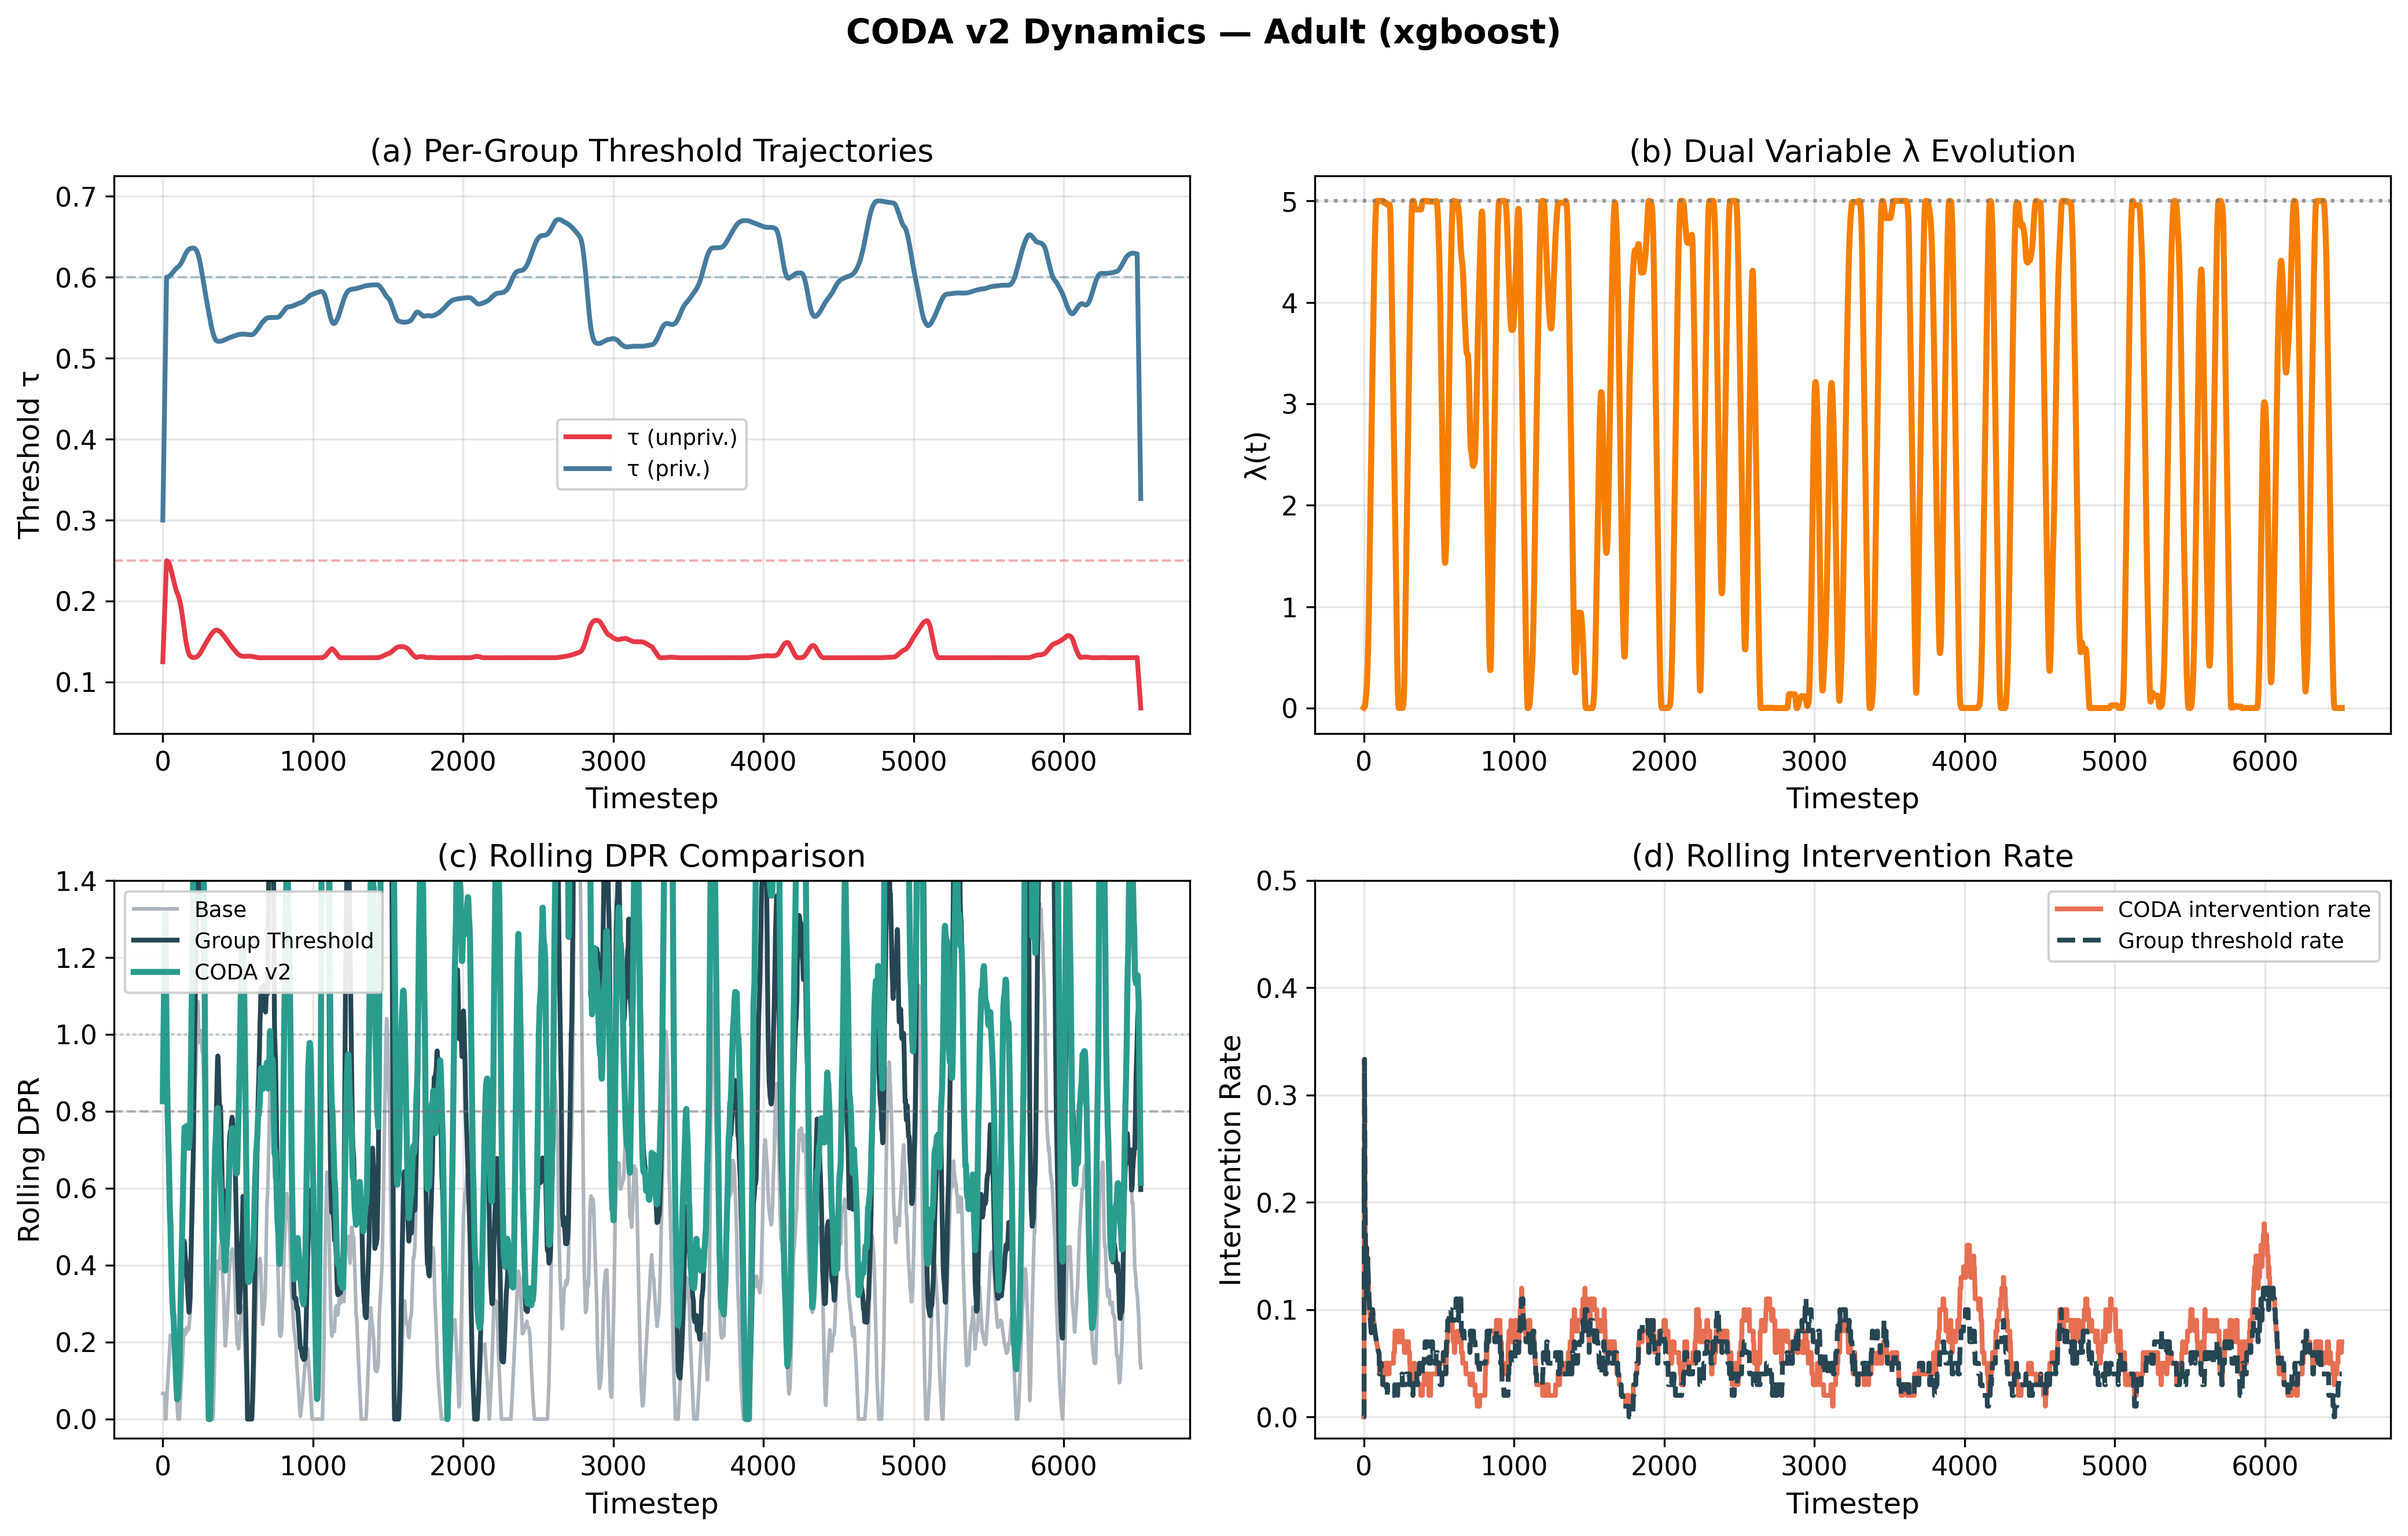
\includegraphics[width=\textwidth]{figures/coda_dynamics_combined_adult.png}
    \caption{CODA v2 dynamics on Adult (XGBoost, seed 42). (a) Per-group threshold trajectories showing asymmetric adaptation. (b) Dual variable $\lambda(t)$ evolution showing active constraint enforcement. (c) Rolling DPR comparison: CODA (teal) achieves consistently higher DPR than Group Threshold (dark) and Base Model (grey). (d) Rolling intervention rate confirming efficient, targeted corrections.}
    \label{fig:dynamics_adult}
\end{figure*}

\begin{figure*}[t]
    \centering
    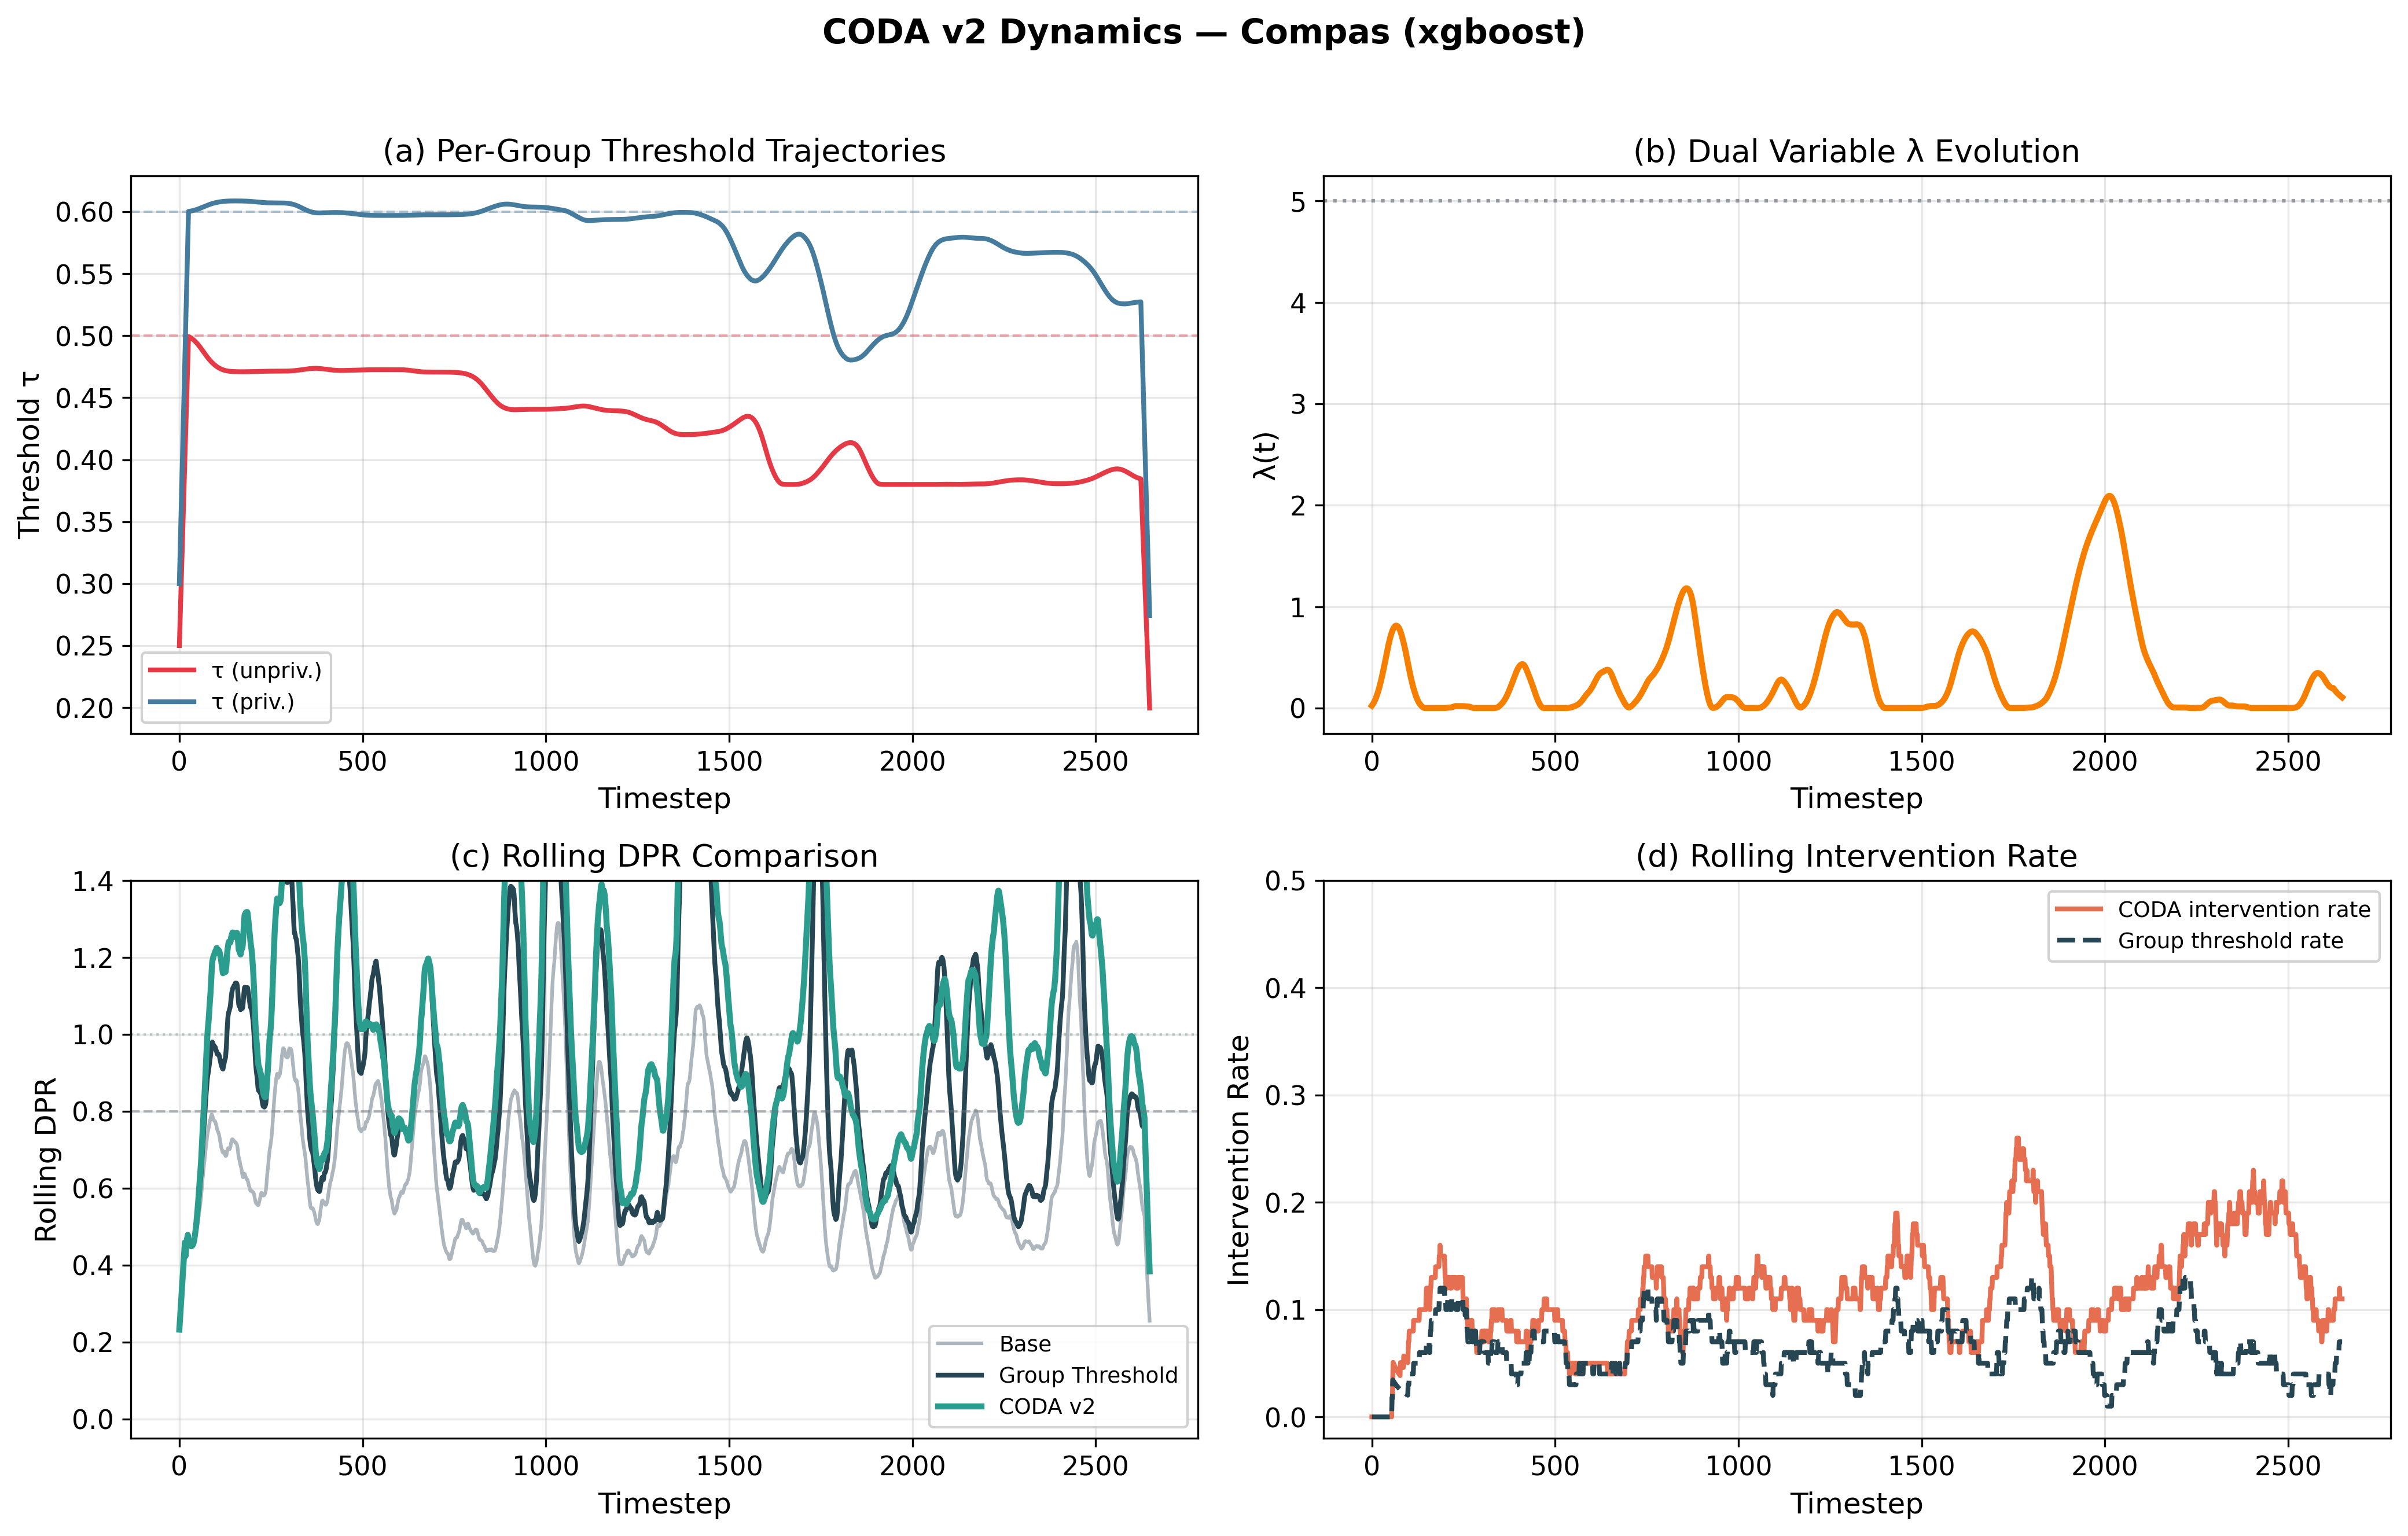
\includegraphics[width=\textwidth]{figures/coda_dynamics_combined_compas.png}
    \caption{CODA v2 dynamics on COMPAS (XGBoost, seed 42). The threshold trajectories in (a) show clean convergence---the unprivileged group threshold rises while the privileged group threshold decreases, leading to near-perfect DPR in (c). The dual variable $\lambda$ in (b) remains mostly near zero, indicating CODA achieves fairness with minimal corrective pressure.}
    \label{fig:dynamics_compas}
\end{figure*}

Key observations from the dynamics plots:
\begin{itemize}
    \item \textbf{Asymmetric adaptation}: On Adult (Figure~\ref{fig:dynamics_adult}a), the privileged group threshold (blue) rises from 0.60 to 0.65--0.70, while the unprivileged group threshold (red) drops from 0.25 to 0.12--0.15. This asymmetry directly creates the DPR improvement.
    \item \textbf{Active constraint enforcement}: The dual variable $\lambda$ on Adult (Figure~\ref{fig:dynamics_adult}b) oscillates between 0 and the cap ($\lambda_{\text{cap}} = 5.0$), indicating continuous, active fairness enforcement. On COMPAS (Figure~\ref{fig:dynamics_compas}b), $\lambda$ remains near zero, indicating CODA achieves fairness easily on this dataset.
    \item \textbf{Convergent behavior}: On COMPAS, the group thresholds converge toward each other over time, consistent with CODA finding an equilibrium where DPR $\approx 1.0$.
    \item \textbf{Intervention efficiency}: Both datasets show CODA's intervention rate tracking close to Group Threshold's rate (5--10\%), confirming that the online adaptation does not introduce excessive overrides.
\end{itemize}

\subsection{Hyperparameter Sensitivity}
\label{sec:sensitivity}

To assess robustness to hyperparameter choices, we sweep each of CODA's six hyperparameters one-at-a-time while holding all others at their validated defaults, evaluating on Adult and COMPAS with XGBoost across 3 seeds (6 runs per setting). Figure~\ref{fig:sensitivity} visualizes the results, and Table~\ref{tab:sensitivity} summarizes the DPR range observed for each hyperparameter.

\begin{figure*}[t]
    \centering
    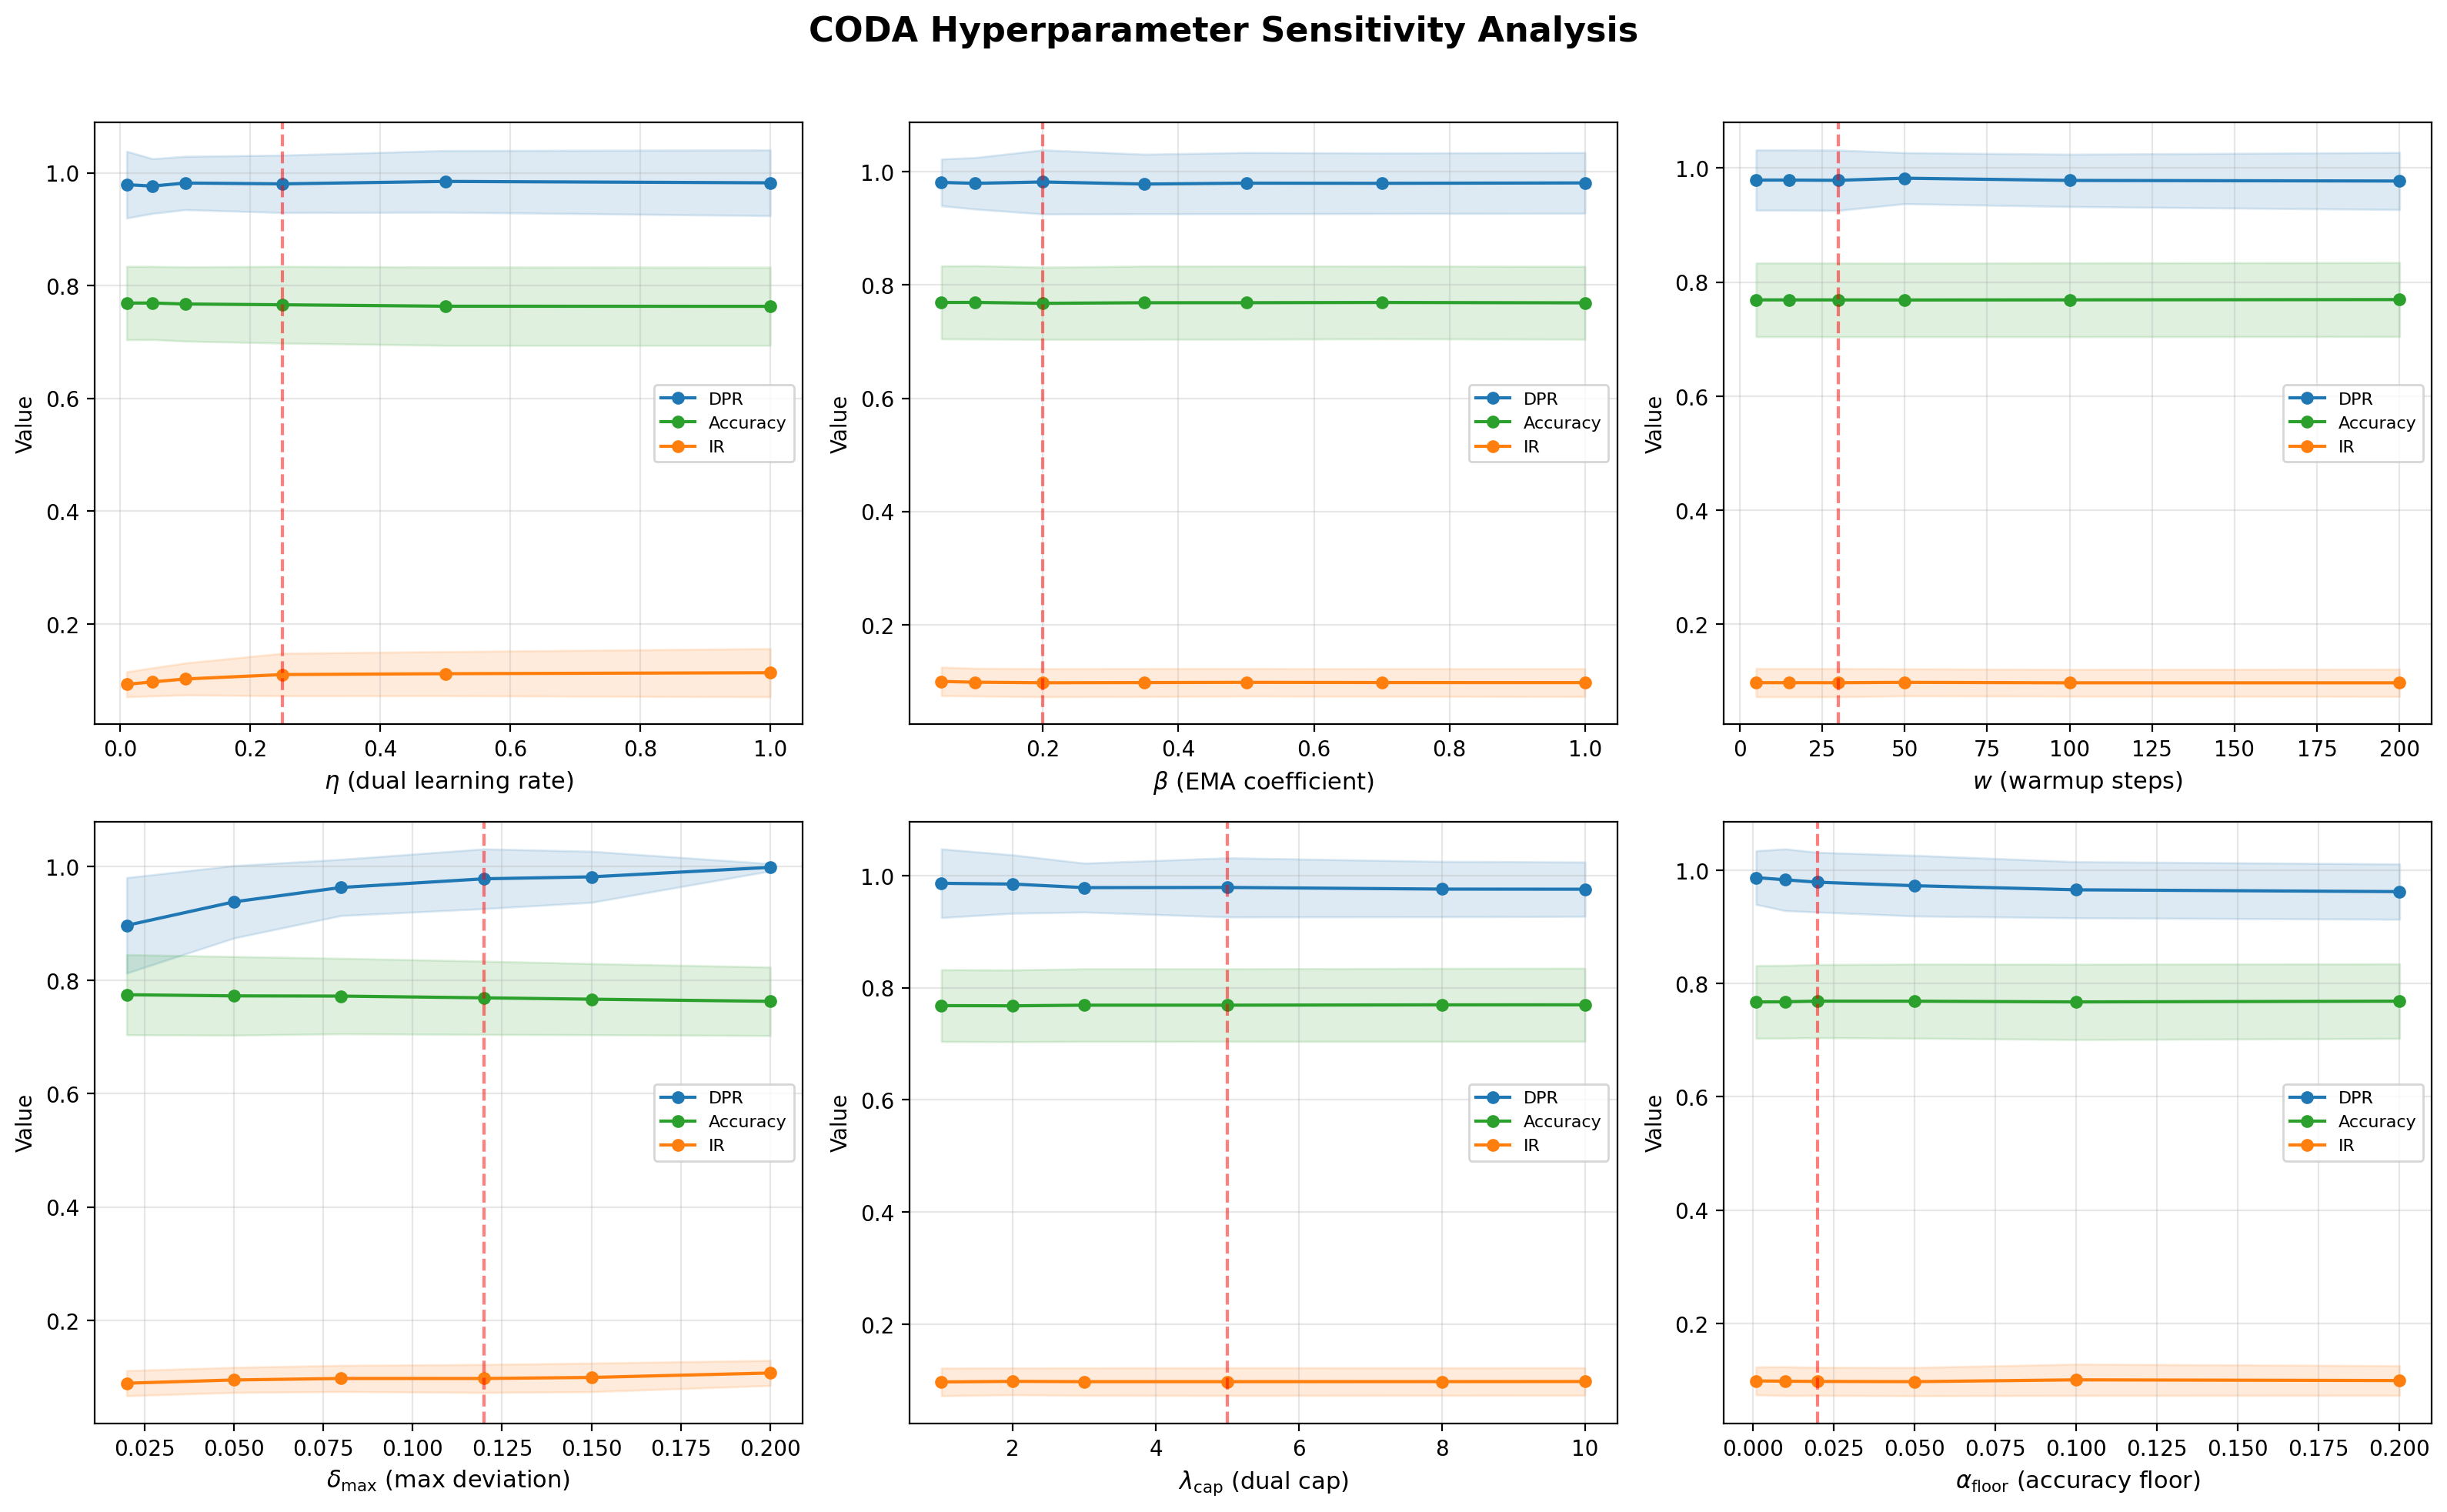
\includegraphics[width=\textwidth]{figures/sensitivity_plot.png}
    \caption{Hyperparameter sensitivity analysis. Each panel sweeps one hyperparameter while holding others at defaults (red dashed line). Blue: DPR, green: accuracy, orange: intervention rate. Shaded regions show 95\% CIs. CODA is robust to 5 of 6 hyperparameters; only $\delta_{\max}$ (max deviation) has a meaningful effect.}
    \label{fig:sensitivity}
\end{figure*}

\begin{table}[t]
\centering
\caption{Hyperparameter sensitivity: DPR range across the full sweep of each hyperparameter. Smaller range indicates lower sensitivity.}
\label{tab:sensitivity}
\small
\begin{tabular}{@{}lcccc@{}}
\toprule
Hyperparameter & Sweep Range & DPR Min & DPR Max & $\Delta$DPR \\
\midrule
$\eta$ (dual LR) & [0.01, 1.0] & 0.977 & 0.985 & 0.008 \\
$\beta$ (EMA coeff.) & [0.05, 1.0] & 0.978 & 0.981 & 0.003 \\
$w$ (warmup) & [5, 200] & 0.977 & 0.982 & 0.005 \\
$\lambda_{\text{cap}}$ (dual cap) & [1.0, 10.0] & 0.976 & 0.986 & 0.010 \\
$\alpha_{\text{floor}}$ (acc.\ floor) & [0.001, 0.2] & 0.962 & 0.987 & 0.025 \\
\midrule
$\delta_{\max}$ (max deviation) & [0.02, 0.20] & \textbf{0.897} & \textbf{0.999} & \textbf{0.102} \\
\bottomrule
\end{tabular}
\end{table}

\textbf{CODA is robust to 5 of 6 hyperparameters.} The dual learning rate $\eta$, EMA coefficient $\beta$, warmup steps $w$, dual cap $\lambda_{\text{cap}}$, and accuracy floor $\alpha_{\text{floor}}$ each produce $\leq 2.5$ percentage point DPR variation across their entire sweep ranges. This is visible in Figure~\ref{fig:sensitivity} as nearly flat lines across each panel. The sole exception is the maximum deviation bound $\delta_{\max}$, which controls how far thresholds can drift from their calibrated initialization. At $\delta_{\max} = 0.02$, DPR drops to 0.897 because CODA cannot adapt thresholds sufficiently; at $\delta_{\max} = 0.20$, DPR reaches 0.999 but accuracy decreases by 1.2pp. This trade-off is expected and interpretable: $\delta_{\max}$ directly governs the capacity for adaptation. The default $\delta_{\max} = 0.12$ sits at the knee of this curve, providing strong DPR (0.979) with minimal accuracy cost.

% ============================================================
\section{Discussion}
\label{sec:discussion}
% ============================================================

\paragraph{When does CODA help most?}
Our results reveal a clear pattern: CODA provides the largest improvements on datasets with \emph{severe initial bias} (Adult: base DPR = 0.296) and \emph{sufficient data} for online adaptation to accumulate signal. On small datasets (German Credit, $n=200$ test), CODA gracefully degrades to static thresholding. This suggests CODA is most valuable in production deployment settings where data streams are large and ongoing.

\paragraph{The accuracy-fairness trade-off.}
CODA consistently trades 0.4--1.0\% accuracy for 4--13pp DPR improvement. This trade-off is favorable: in regulated domains (e.g., lending under the Equal Credit Opportunity Act), fairness compliance is a hard constraint, and small accuracy costs are acceptable.

\paragraph{Practical deployment considerations.}
CODA requires no access to true labels at deployment time---it adapts using only the observed scores and group attributes. This makes it suitable for real-world settings where ground truth is delayed (e.g., loan default takes years to observe) or unavailable. The rolling window size ($w=200$) and warmup period are configurable to match the expected data rate.

\paragraph{Intervention rate trade-off.}
CODA's intervention rate (0.080) is marginally higher than Group Threshold's (0.069), but the 95\% confidence intervals overlap ($[0.062, 0.098]$ vs.\ $[0.052, 0.085]$), indicating the difference is not statistically significant at conventional levels. In settings where intervention rate must be minimized---for example, to limit override liability in automated lending---the grid search objective (Eq.~\ref{eq:gridsearch}) can be adjusted to increase the IR penalty coefficient from 0.5 to a higher value, trading fairness improvement for lower intervention frequency. CODA's modular design makes this trade-off explicit and configurable.

\paragraph{Deployment context and group attribute observability.}
CODA assumes that the protected group attribute $a_t$ is observed at decision time. This assumption warrants careful examination across application domains:
\begin{itemize}
    \item \textbf{Lending (U.S.):} Under the Equal Credit Opportunity Act (ECOA), race and sex cannot be used in credit decisions but are often available via Bayesian Improved Surname Geocoding (BISG) for fair lending monitoring. CODA is compatible with proxy-based group assignment; however, proxy noise would widen the rolling DPR estimator's variance, potentially requiring larger window sizes.
    \item \textbf{Criminal justice:} Race is typically recorded in presentence reports and booking data. CODA's threshold adjustments operate on model scores, not directly on the protected attribute, mitigating some disparate treatment concerns.
    \item \textbf{Hiring:} Gender and race may be self-reported and optional. When group labels are missing for a fraction of instances, CODA's warmup mechanism provides a natural safeguard: adaptation activates only after sufficient observations from each group.
    \item \textbf{EU context:} Under GDPR Article 9, processing of special category data (including race and ethnicity) requires explicit legal basis. In jurisdictions where protected attributes cannot legally be used even for fairness-improving interventions, CODA is not directly deployable without regulatory accommodation.
\end{itemize}
We acknowledge that the sociotechnical landscape of group attribute availability is complex and jurisdiction-dependent, and that deployment of any threshold-adjustment method requires engagement with the specific regulatory and ethical context of the application domain.

\paragraph{Limitations.}
(i) CODA optimizes for demographic parity ratio. Extending the dual update to simultaneously enforce equalized odds is possible but requires tracking per-group confusion matrices, which demands more data per group. (ii) The current multi-group extension uses an extremal-pair update, which may be suboptimal when multiple intermediate groups contribute to the DPR gap. (iii) CODA's theoretical guarantees hold under the assumption that the rolling DPR estimator is unbiased, which requires sufficient group representation in each window. (iv) CODA has six tunable hyperparameters ($\eta$, $\beta$, $w$, $\delta_{\max}$, $\lambda_{\text{cap}}$, $\alpha_{\text{floor}}$); our sensitivity analysis (Section~\ref{sec:sensitivity}) shows that 5 of 6 are robust, but $\delta_{\max}$ requires domain-appropriate selection.

% ============================================================
\section{Conclusion}
\label{sec:conclusion}
% ============================================================

We introduced CODA, an online fairness controller that bridges the gap between static post-processing and adaptive deployment-time fairness enforcement. By formulating threshold adaptation as online constrained optimization and solving it via primal-dual updates, CODA achieves $O(\sqrt{T})$ cumulative fairness violation---a worst-case guarantee that static thresholds cannot match under adversarial stream ordering. Our comprehensive evaluation across 5 datasets, ablation studies, and multi-group extensions demonstrates that CODA is both theoretically principled and practically effective. The order stress experiments (Table~\ref{tab:orderstress}) provide particularly compelling evidence: while Universal RL achieves marginally higher mean DPR under benign ordering, it collapses catastrophically under adversarial ordering (DPR $> 2.3$ on Adult), whereas CODA remains stable (DPR range $\leq 0.15$). The multi-group extension, which reduces the DPR gap by 31\% on a 5-group racial fairness task, represents a further advance for real-world applications where protected attributes are inherently multi-valued.

\paragraph{Future work.}
Promising directions include: (i) extending CODA to enforce multiple fairness constraints simultaneously (e.g., DPR and equalized odds) via multi-dimensional dual variables; (ii) incorporating distribution shift detection to dynamically adjust the rolling window size; and (iii) evaluating CODA in true online production settings with concept drift.

% ============================================================
% BIBLIOGRAPHY
% ============================================================
\bibliographystyle{plain}

\begin{thebibliography}{30}

\bibitem{hardt2016equality}
M.~Hardt, E.~Price, and N.~Srebro.
\newblock Equality of opportunity in supervised learning.
\newblock In {\em Advances in Neural Information Processing Systems (NeurIPS)}, pages 3315--3323, 2016.

\bibitem{pleiss2017fairness}
G.~Pleiss, M.~Raghavan, F.~Wu, J.~Kleinberg, and K.~Q. Weinberger.
\newblock On fairness and calibration.
\newblock In {\em Advances in Neural Information Processing Systems (NeurIPS)}, pages 5680--5689, 2017.

\bibitem{menon2018cost}
A.~K. Menon and R.~C. Williamson.
\newblock The cost of fairness in binary classification.
\newblock In {\em Proceedings of the 1st Conference on Fairness, Accountability and Transparency (FAccT)}, pages 107--118, 2018.

\bibitem{mahdavi2012trading}
M.~Mahdavi, R.~Jin, and T.~Yang.
\newblock Trading regret for efficiency: Online convex optimization with long term constraints.
\newblock {\em Journal of Machine Learning Research}, 13:2503--2528, 2012.

\bibitem{hazan2016introduction}
E.~Hazan.
\newblock Introduction to online convex optimization.
\newblock {\em Foundations and Trends in Optimization}, 2(3-4):157--325, 2016.

\bibitem{shalev2012online}
S.~Shalev-Shwartz.
\newblock Online learning and online convex optimization.
\newblock {\em Foundations and Trends in Machine Learning}, 4(2):107--194, 2012.

\bibitem{barocas2016big}
S.~Barocas and A.~D. Selbst.
\newblock Big data's disparate impact.
\newblock {\em California Law Review}, 104:671--732, 2016.

\bibitem{chouldechova2017fair}
A.~Chouldechova.
\newblock Fair prediction with disparate impact: A study of bias in recidivism prediction instruments.
\newblock {\em Big Data}, 5(2):153--163, 2017.

\bibitem{caton2024fairness}
S.~Caton and C.~Haas.
\newblock Fairness in machine learning: A survey.
\newblock {\em ACM Computing Surveys}, 56(7):1--38, 2024.

\bibitem{mehrabi2021survey}
N.~Mehrabi, F.~Morstatter, N.~Saxena, K.~Lerman, and A.~Galstyan.
\newblock A survey on bias and fairness in machine learning.
\newblock {\em ACM Computing Surveys}, 54(6):1--35, 2021.

\bibitem{singh2024fairness}
A.~Singh, D.~Raghu, S.~Srivastava, and P.~Agrawal.
\newblock Supervised algorithmic fairness in distribution shifts: A survey.
\newblock In {\em Proceedings of the International Joint Conference on Artificial Intelligence (IJCAI)}, 2024.

\bibitem{chen2025fairnessdrift}
Y.~Chen et~al.
\newblock Emerging algorithmic bias: Fairness drift as the next dimension of model maintenance and sustainability.
\newblock {\em npj Digital Medicine}, 8(1):1--8, 2025.

\bibitem{rezaei2021robust}
A.~Rezaei, A.~Liu, K.~Memarrast, and B.~D. Ziebart.
\newblock Robust fairness under covariate shift.
\newblock In {\em Proceedings of the AAAI Conference on Artificial Intelligence}, pages 9419--9427, 2021.

\bibitem{gillen2018online}
S.~Gillen, C.~Jung, M.~Kearns, and A.~Roth.
\newblock Online learning with an unknown fairness metric.
\newblock In {\em Advances in Neural Information Processing Systems (NeurIPS)}, pages 2600--2609, 2018.

\bibitem{blum2018preserving}
A.~Blum, S.~Gunasekar, T.~Lykouris, and N.~Srebro.
\newblock On preserving non-discrimination when combining expert advice.
\newblock In {\em Advances in Neural Information Processing Systems (NeurIPS)}, pages 8376--8387, 2018.

\bibitem{roh2021fairbatch}
Y.~Roh, K.~Lee, S.~E. Whang, and C.~Suh.
\newblock FairBatch: Batch selection for model fairness.
\newblock In {\em International Conference on Learning Representations (ICLR)}, 2021.

\bibitem{zhang2020fairness}
X.~Zhang and M.~Shah.
\newblock Fair decision-making under uncertainty.
\newblock In {\em IEEE International Conference on Data Mining (ICDM)}, pages 886--895, 2020.

\bibitem{kearns2018preventing}
M.~Kearns, S.~Neel, A.~Roth, and Z.~S. Wu.
\newblock Preventing fairness gerrymandering: Auditing and learning for subgroup fairness.
\newblock In {\em Proceedings of the 35th International Conference on Machine Learning (ICML)}, pages 2564--2572, 2018.

\bibitem{hebert2018multicalibration}
U.~H{\'e}bert-Johnson, M.~Kim, O.~Reingold, and G.~Rothblum.
\newblock Multicalibration: Calibration for the (computationally-identifiable) masses.
\newblock In {\em Proceedings of the 35th International Conference on Machine Learning (ICML)}, pages 1939--1948, 2018.

\bibitem{biddle2006adverse}
D.~Biddle.
\newblock {\em Adverse Impact and Test Validation: A Practitioner's Guide to Valid and Defensible Employment Testing}.
\newblock Gower Publishing, 2nd edition, 2006.

\bibitem{dua2019uci}
D.~Dua and C.~Graff.
\newblock {UCI} machine learning repository, 2019.
\newblock \url{http://archive.ics.uci.edu/ml}.

\bibitem{angwin2016machine}
J.~Angwin, J.~Larson, S.~Mattu, and L.~Kirchner.
\newblock Machine bias.
\newblock {\em ProPublica}, May 2016.

\bibitem{moro2014data}
S.~Moro, P.~Cortez, and P.~Rita.
\newblock A data-driven approach to predict the success of bank telemarketing.
\newblock {\em Decision Support Systems}, 62:22--31, 2014.

\bibitem{recruitment2023}
Synthetic Recruitment Dataset.
\newblock Kaggle, 2023.
\newblock \url{https://www.kaggle.com/datasets/}.

\end{thebibliography}

\end{document}
